\documentclass{article}
% \renewcommand{\thesection}{\arabic{section}}
% \setcounter{tocdepth}{1}
% index
% \usepackage{imakeidx}
% \makeindex%[title=Index, intoc]
% glossary
% \usepackage{glossaries}
% \makeglossaries
% geometry formatting
\usepackage{authblk}
\usepackage[utf8]{inputenc}
\usepackage[margin=0.75in]{geometry}
\usepackage{parskip, setspace}
\setstretch{1.15}
% math formatting
\usepackage{amsmath, amsfonts, braket}
% \numberwithin{equation}{section}
% rich text
\usepackage{graphicx, caption}
\usepackage{hyperref}
% \usepackage{xcolor}
\hypersetup{
    colorlinks=true,
    linkcolor=black,  
    urlcolor=blue,
    citecolor=blue,
    pdftitle={A Survey of Computational Physics},
    pdfpagemode=FullScreen,
}
% bibliography
\usepackage{biblatex}
\addbibresource{bib.bib}

% \renewcommand{\arraystretch}{1.5} % give a little more space in table

\title{CS 530: High-Performance Computing \\ Seminar 2: Quantum Computing}
\author{Nathan Chapman}
\affil{Department of Computer Science \\ Central Washington University}
\date{\today}

\begin{document}

\maketitle

\tableofcontents

\section{History of Quantum Computation \& Information}

\section{Quantum Bits}

    \begin{itemize}
        \item The bit and qubit is the most fundamental concept of information
        \item A classical bit has a state: either 0 or 1
        \item A quantum bit   has a state: $\ket{0}, \ket{1}, \alpha \ket{0} + \beta \ket{1}$ for complex $\alpha, \beta$ such that $|\alpha|^2 + |\beta|^2 = 1$
        \item The state of a qubit is a unit vector in a two-dimensional complex vector space.  In other words, qubits similar to are unit quarternions.
        \item $\ket{0}, \ket{1}$ are orthonormal and form computational basis states
        \item Can't directly measure $\alpha, \beta$
        \item Example: a ``quantim coin'' with state $\ket{+} = \frac{1}{\sqrt{2}} \ket{0} + \frac{1}{\sqrt{2}} \ket{1}$ and 50-50 probability
        \item Can write $\ket{\psi} = e^{i \gamma} \left(\cos \left( \frac{\theta}{2} \right) \ket{0} + e^{i \phi} \sin \left( \frac{\theta}{2} \right) \ket{0} \right)$
        \item Because $e^{i \gamma}$ has no observable effect, we can reduced the above to $\ket{\psi} = \cos \left( \frac{\theta}{2} \right) \ket{0} + e^{i \phi} \sin \left( \frac{\theta}{2} \right) \ket{0}$
        \item While a qubit can only measure to be 0 or 1, until measurement there is ``hidden information'' encoded in $\alpha$ and $\beta$.
    \end{itemize}

    \subsection{Multiple Qubits}

        \begin{itemize}
            \item For two qubits, there are $2^2$ computational basis states where $\ket{\psi} = \alpha_{00} \ket{00} + \alpha_{01} \ket{01} + \alpha_{10} \ket{10} + \alpha_{11} \ket{11}$ where $\alpha \in \mathbb{C}$ such that $\sum |\alpha|^2 = 1$
            \item Could measure just one qubit, possbly as zero, resulting in the re-normalized post-measurement state $\ket{\psi_0} = \frac{\alpha_{00} \ket{00} + \alpha_{01} \ket{01}}{\sqrt{|\alpha_{00}|^2 + |\alpha_{01}|^2}}$
            \item Bell state or EPR state $\frac{1}{\sqrt{2}} \ket{00} + \frac{1}{\sqrt{2}} \ket{11}$
            \item Measure one of the bits in the Bell state and the second one must be the same with a 50\% chance
            \item Extend to $N$ qubits for a state with $2^N$ amplitudes
            \item ? If $N = 500$, a classical computer could never store $2^500$ bits, as that is more than the predicted number of atoms in the universe
        \end{itemize}

\section{Quantum Computation}

        \begin{itemize}
            \item Classical computers are built with electric circuits consisting of wire and logic gates
            \item Quantum computers are built with quantum circuits consisting of wires and quantum gates
        \end{itemize}

    \subsection{Quantum Gates}

        \subsubsection{Single Qubit Gates}

            \begin{itemize}
                \item Only non-trivial example is the NOT gate defined by its truth table $0 \to 1$ and $1 \to 0$.
                \item Physically, there needs to exist some process by which we can ``flip'' the qubit.
                \item If $\ket{\psi} = \alpha \ket{0} + \beta \ket{1}$, then $\ket{\lnot\psi} = \beta \ket{0} + \alpha \ket{1}$ (where $\lnot$ represents logical negation)
                \item In a basis representation, $\ket{\psi} = \begin{bmatrix} \alpha \\ \beta \end{bmatrix} \implies \ket{\lnot\psi} = \begin{bmatrix} \beta \\ \alpha \end{bmatrix}$
                \item The mathematical action of the NOT operation can thus be represented by the matrix $X = \begin{bmatrix}
                    0 & 1 \\
                    1 & 0 
                \end{bmatrix}$
                \item Yielding $X \begin{bmatrix} \alpha \\ \beta \end{bmatrix} = \begin{bmatrix} \beta \\ \alpha \end{bmatrix}$
                \item Quantum gates on a single qubit can be represented by a $2 \times 2$ matrix
                \item Because the result of applying a quantum gate $U$ to a normalized quantum state is itself a normalized quantum state, the matrix representation of the quantum gate said to be \emph{unitary} in the sense that $U^\dagger U = I$, where $U^\dagger$ is the \emph{adjoint} of the operator $U$ or conjugate-transpose of the matrix representation of $U$, and $I$ is the $2 \times 2$ identity matrix.
                \item It turns out unitarity is the only constraint on quantum gates
                \item Unlike in classical logic, there are multiple non-trivial single-qubit gates.
                \item The $Z$ gate effectively just flips the sign on the $\ket{1}$ state by defining $Z \equiv \begin{bmatrix}
                    1 & 0 \\
                    0 & -1
                \end{bmatrix}$
                \item The \emph{Hadamard} gate $H$ defined as $H \equiv \dfrac{1}{\sqrt{2}} \begin{bmatrix}
                    1 & 1 \\
                    1 & -1
                \end{bmatrix}$
                \item The Hadamard gate can be thought of as the ``square root'' of the NOT gate, though $H^2 = I \neq X$, because 
                \begin{align}
                    H \ket{0} = \frac{1}{\sqrt{2}} \left(\ket{0} + \ket{1}\right) \\
                    H \ket{1} = \frac{1}{\sqrt{2}} \left(\ket{0} - \ket{1}\right)
                \end{align}
                each of which transforms its input ``halfway'' toward the other.
                \begin{figure}[h]
                    \centering
                    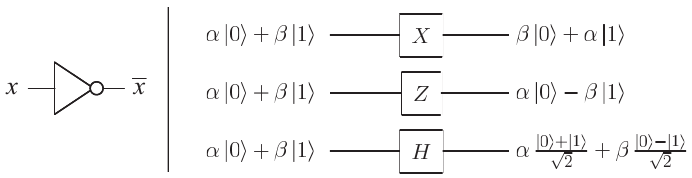
\includegraphics[width=0.66\textwidth]{images/single_circuits.png}
                    \caption{A comparison between logic gates that can act on a single classical or quantum bit.}
                \end{figure}
                \item It turns out that there are infinitely many unitary single-qubit quantum gates.  Each of these gates $U$ can be represented by specifying real-valued $\alpha, \beta, \gamma, \delta$ and 
                \begin{equation}
                    U = e^{i \alpha} 
                    \begin{bmatrix}
                        e^{-i \beta /2} & 0 \\
                        0               & e^{i \beta / 2}
                    \end{bmatrix} 
                    \begin{bmatrix}
                        \cos(\gamma /2) & - \sin(\gamma / 2) \\
                        \sin(\gamma / 2) & \cos(\gamma / 2)
                    \end{bmatrix}
                    \begin{bmatrix}
                        e^{-i \delta /2} & 0 \\
                        0               & e^{i \delta / 2}
                    \end{bmatrix} 
                \end{equation}
                \item This decompisition means that a quantum gate can be thought of as applying a sequence of rotations in different planes
            \end{itemize}

        \subsubsection{Multi-Qubit Gates}

            

    \subsection{Quantum Circuits}

    \subsection{Examples}

        \subsubsection{Bell States}

        \subsubsection{Quantum Teleportation}

\section{Quantum Algorithms}

    \subsection{Examples}

        \subsubsection{The Quantum Fourier Transform}

        \subsubsection{The Quantum Search Algorithm}

\section{Quantum Information}

    \subsection{Quantum Cryptography}

\newpage
\nocite{*}
\printbibliography

\end{document}